\documentclass[a4paper,12pt]{ctexart}

\usepackage{geometry}
\geometry{a4paper, left=2.5cm, right=2.5cm, top=2.5cm, bottom=2.5cm}

\usepackage{amsmath}
\usepackage{caption}
\usepackage{graphicx}
\usepackage{listings}
\usepackage{xcolor}
\usepackage{fontspec}
\usepackage{url}

\setmainfont{Microsoft YaHei}

\setkeys{Gin}{width=\textwidth, keepaspectratio}

\lstset{
	basicstyle=\footnotesize\ttfamily,
	frame=single,
	numbers=none,
	backgroundcolor=\color{gray!5},
	breaklines=true,
	breakatwhitespace=false,
	columns=flexible,
	xleftmargin=4pt,
	xrightmargin=4pt,
	breakindent=1em
}



\begin{document}
	
	\title{系统开发工具基础 第二周实验报告}
	\author{涂睿昕---25020007115}
	\maketitle
	
	\section{实验概述}
	 本次实验为系统开发工具基础第二周课上实验，实验环境为VirtualBox中的Ubuntu虚拟机。本次完成四项课上实验：进程与信号控制、IDE语义重构开发反馈、调试器定位程序缺陷、性能分析与程序优化。实验主要练习Linux进程与信号、Shell任务调度、Python调试器、性能剖析工具、cgroups资源隔离、ulimit资源软限制，掌握多终端协同观测、内核资源管控与命令行性能排查的基本流程。
	
	\section{课上实验题目}
	\subsection{q05：控制一个可清理的后台任务}
	\subsubsection{题目要求}
     编写worker.sh脚本，实现信号捕获逻辑；前台启动脚本，将标准输出、标准错误分别重定向至日志文件；使用\texttt{Ctrl‑Z}挂起任务，再使用\texttt{bg}将任务转入后台继续运行；通过\texttt{jobs -p}获取进程PID，禁止手工抄写PID；向进程发送SIGTERM信号，禁止使用kill -9；验证cleanup.log中输出CLEAN\_EXIT，确认任务正常退出。
	
	\subsubsection{实现过程与关键命令}
	\begin{lstlisting}
		cd ~/sdt-course/week2/q05
		cat > worker.sh <<'EOF'
		#!/usr/bin/env bash
		trap 'echo CLEAN_EXIT >> cleanup.log; exit 0' TERM INT
		n=0
		while true; do
		echo "$n"
		n=$((n+1))
		sleep 1
		done
		EOF
		chmod +x worker.sh
		
		./worker.sh > stdout.log 2> stderr.log
		# Ctrl‑Z 挂起任务
		bg
		jobs
		jobs -p
		kill -TERM 10098
		jobs
		cat cleanup.log
	\end{lstlisting}
	
	\subsubsection{运行结果}
     执行结束后，cleanup.log文件内存在字符串\texttt{CLEAN\_EXIT}，进程收到信号后正常退出，无进程残留；stdout.log持续输出递增的数字序列，stderr.log为空。
	\begin{lstlisting}
		^Z      
		[1]+  已停止               ./worker.sh > stdout.log 2> stderr.log
		
		[1]+ ./worker.sh > stdout.log 2> stderr.log &
		
		[1]+  运行中               ./worker.sh > stdout.log 2> stderr.log &
		
		10098
		
		[1]+  已完成               ./worker.sh > stdout.log 2> stderr.log
		
		CLEAN_EXIT
	\end{lstlisting}
	
	\begin{figure}[htbp]
		\centering
		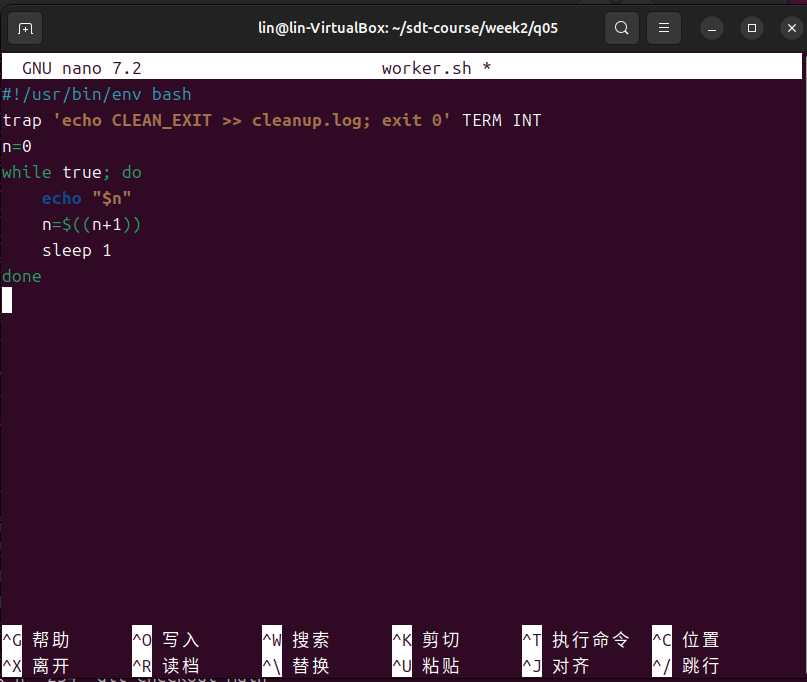
\includegraphics[width=0.9\textwidth]{q5p1.png}
		\caption{q05 worker.sh截图}
		\label{fig.q05_1}
	\end{figure}
	
	\subsubsection{遇到的问题与解决}
    \begin{itemize}
	    \item 问题1：使用\texttt{kill -9}强制杀死进程，trap无法捕获该信号，cleanup.log不会输出清理标记。
    	解决：直接使用kill发送SIGTERM，给予脚本执行trap定义的清理逻辑的机会。
    	\item 问题2：手动复制粘贴PID，不符合题目不手工抄写PID的约束。
    	解决：使用\texttt{jobs -p}获取后台任务PID并赋值给shell变量。
    \end{itemize}
	
	\subsection{q06：语义重构与本地开发反馈}
	\subsubsection{题目要求}
	 创建math\_utils.py、app.py、test\_math\_utils.py三份源码；借助Python语言服务器实现跳转到定义、查找引用；使用重命名符号功能将\texttt{total\_price}同步修改为\texttt{calculate\_total}；临时加入未使用的import语句，使用ruff检测并删除无用导入；执行ruff检查格式化与pytest单元测试，保证全部通过。
	
	\subsubsection{实现过程与关键命令}
	\begin{lstlisting}
		cd ~/sdt-course/week2/q06
		nano # 创建三份python源码文件
		code .
		# VS Code语言服务器：跳转定义（F12）、查找所有引用（shift+F12）
		# 使用重命名符号完成标识符全局替换（F2）
		# 临时添加import os复现未使用导入告警
		ruff check .
		ruff check --fix
		ruff check .
		pytest test_math_utils.py -v
	\end{lstlisting}
	
	\subsubsection{运行结果}
	重命名符号操作后，定义与全部引用位置同步更新；ruff无告警输出；pytest全部测试用例执行PASS。
	\begin{lstlisting}
		I001  [*] Import block is un‑sorted or un‑formatted
		--> app.py:1:1
		1 │ / import os
		2 │ from math_utils import calculate_total
		│ └───────────────────────────────────^
		3 │
		4 │ print(calculate_total(12.5, 4))
		
		help: Organize imports
		1 │ import os
		2 │
		3 │ from math_utils import calculate_total
		
		F401  [*] `os` imported but unused
		--> app.py:1:8
		1 │ import os
		│        ^^
		2 │ from math_utils import calculate_total
		
		help: Remove unused import: `os`
		- import os
		1 │ from math_utils import calculate_total
		
		I001  [*] Import block is un‑sorted or un‑formatted
		--> test_math_utils.py:1:1
		1 │ from math_utils import calculate_total
		│ └────────────────────────────────────^^
		2 │
		3 │ def test_total_price():
		
		help: Organize imports
		2 │
		3 │
		4 │ def test_total_price():
		
		Found 3 errors.
		[*] 3 fixable with the `--fix` option.
		
		Found 2 errors (2 fixed, 0 remaining).
		
		All checks passed!
		
		======================== test session starts ========================
		platform linux -- Python 3.12.3, pytest‑9.1.1, pluggy‑1.6.0
		rootdir: /home/lin/sdt‑course/week2/q06
		collected 1 item
		
		test_math_utils.py .                                                               [100%]
		
		======================== 1 passed in 0.00s ========================
	\end{lstlisting}
	
	\begin{figure}[htbp]
		\centering
		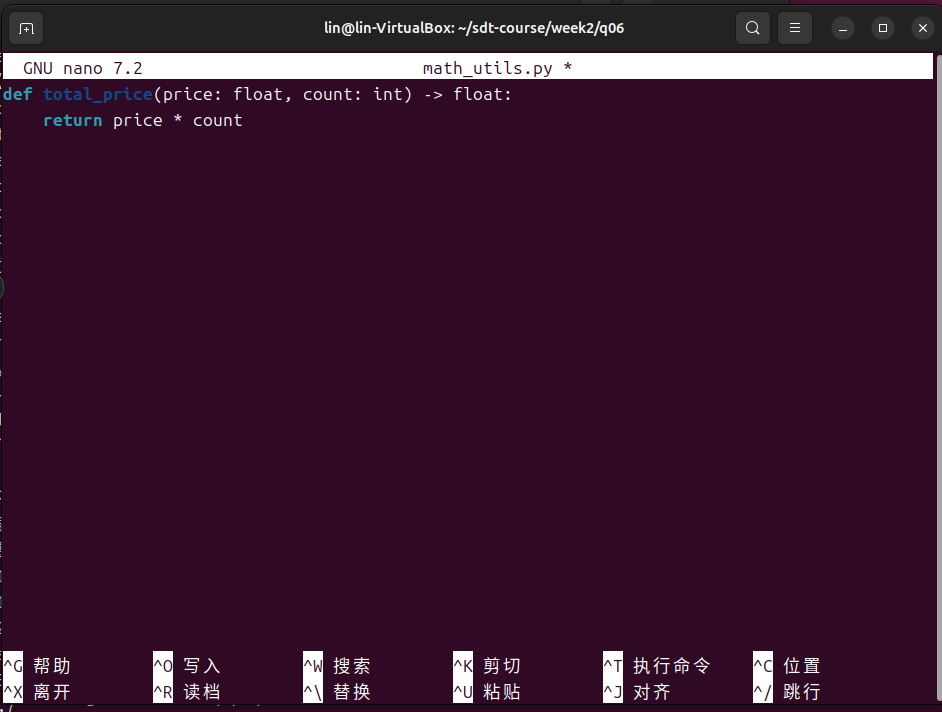
\includegraphics[width=0.9\textwidth]{q6p1.png}
		\caption{q06math\_utils.py截图}
		\label{fig:q06_1}
	\end{figure}
	
	\begin{figure}[htbp]
		\centering
		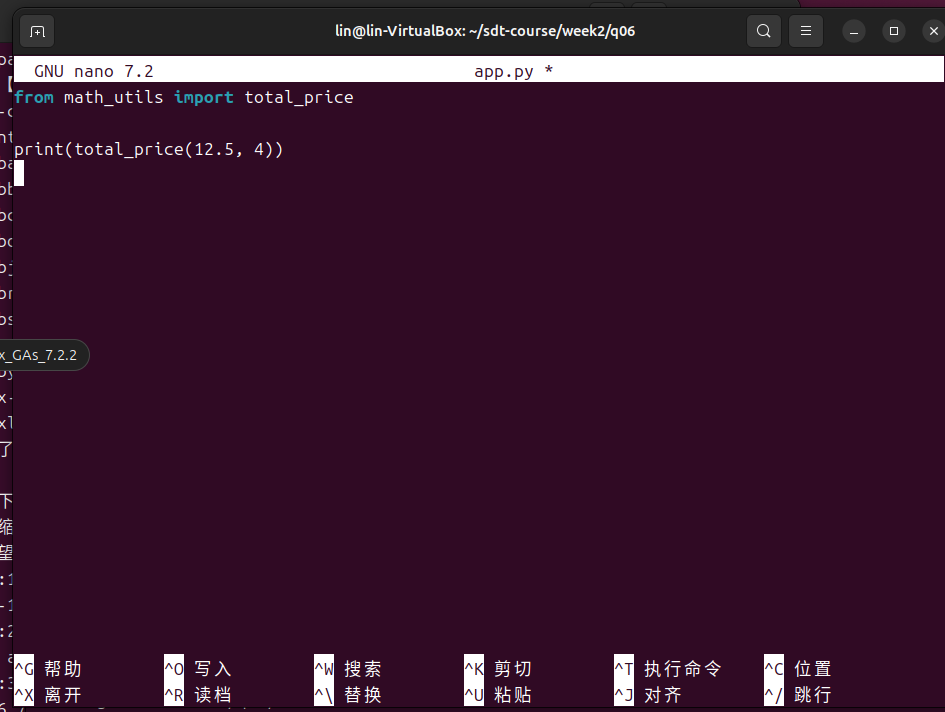
\includegraphics[width=0.9\textwidth]{q6p2.png}
		\caption{q06app.py截图}
		\label{fig:q06_2}
	\end{figure}
	
	\begin{figure}[htbp]
		\centering
		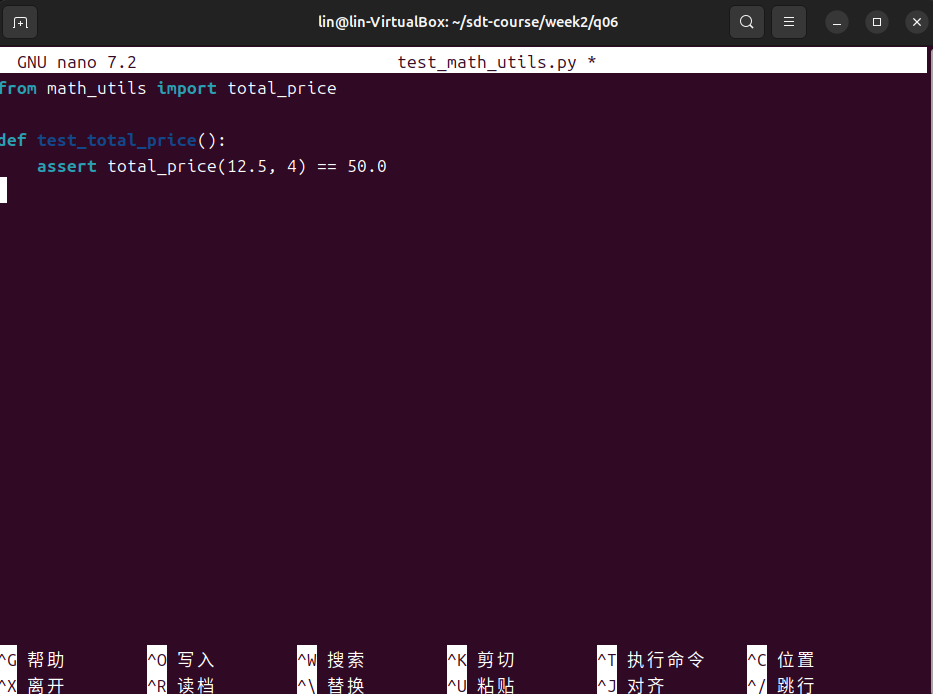
\includegraphics[width=0.9\textwidth]{q6p3.png}
		\caption{q06test\_math\_utils.py截图}
		\label{fig:q06_3}
	\end{figure}
	
	\begin{figure}[htbp]
		\centering
		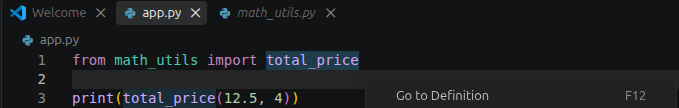
\includegraphics[width=0.9\textwidth]{q6p4.png}
		\caption{q06vscode跳转定义操作截图}
		\label{fig:q06_4}
	\end{figure}
	
	\begin{figure}[htbp]
		\centering
		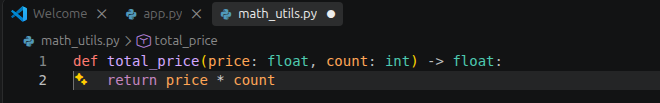
\includegraphics[width=0.9\textwidth]{q6p5.png}
		\caption{q06vscode跳转定义结果截图}
		\label{fig:q06_5}
	\end{figure}
	
	\begin{figure}[htbp]
		\centering
		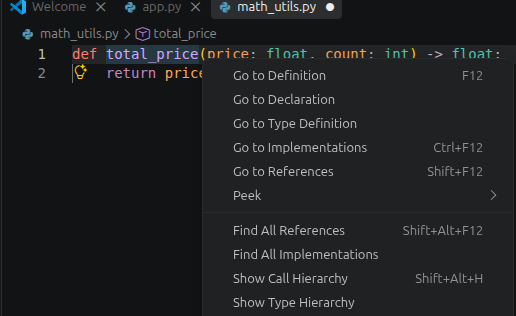
\includegraphics[width=0.9\textwidth]{q6p6.png}
		\caption{q06vscode查找所有引用操作截图}
		\label{fig:q06_6}
	\end{figure}
	
	\begin{figure}[htbp]
		\centering
		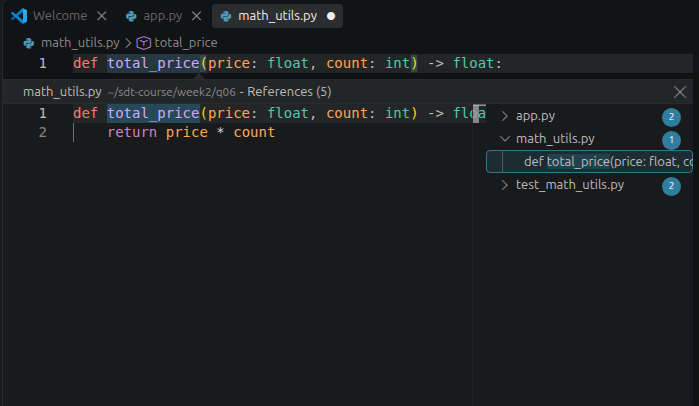
\includegraphics[width=0.9\textwidth]{q6p7.png}
		\caption{q06vscode查找所有引用结果截图}
		\label{fig:q06_7}
	\end{figure}
	
	\begin{figure}[htbp]
		\centering
		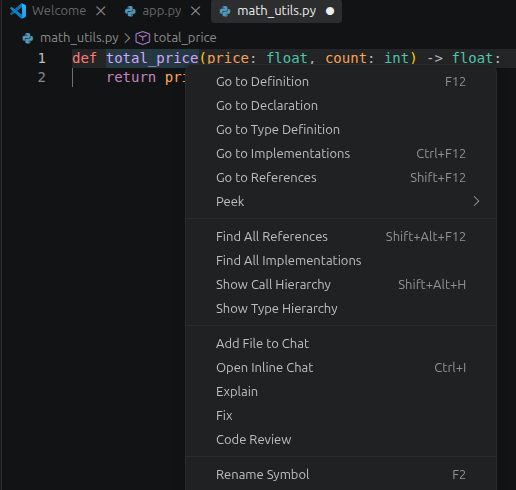
\includegraphics[width=0.9\textwidth]{q6p8.png}
		\caption{q06vscode重命名操作截图1}
		\label{fig:q06_8}
	\end{figure}
	
	\begin{figure}[htbp]
		\centering
		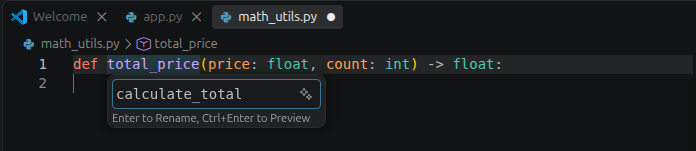
\includegraphics[width=0.9\textwidth]{q6p9.png}
		\caption{q06vscode重命名操作截图2}
		\label{fig:q06_9}
	\end{figure}
	
	\begin{figure}[htbp]
		\centering
		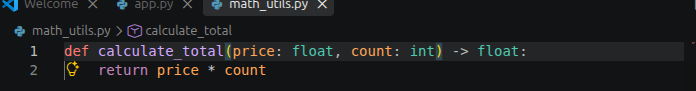
\includegraphics[width=0.9\textwidth]{q6p10.png}
		\caption{q06vscode重命名结果截图1}
		\label{fig:q06_10}
	\end{figure}
	
	\begin{figure}[htbp]
		\centering
		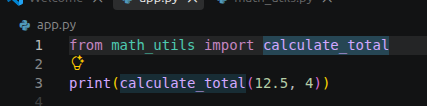
\includegraphics[width=0.9\textwidth]{q6p11.png}
		\caption{q06vscode重命名结果截图2}
		\label{fig:q06_11}
	\end{figure}
	
	\begin{figure}[htbp]
		\centering
		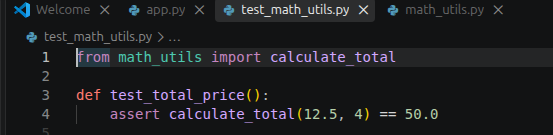
\includegraphics[width=0.9\textwidth]{q6p12.png}
		\caption{q06vscode重命名结果截图3}
		\label{fig:q06_12}
	\end{figure}
	
	\begin{figure}[htbp]
		\centering
		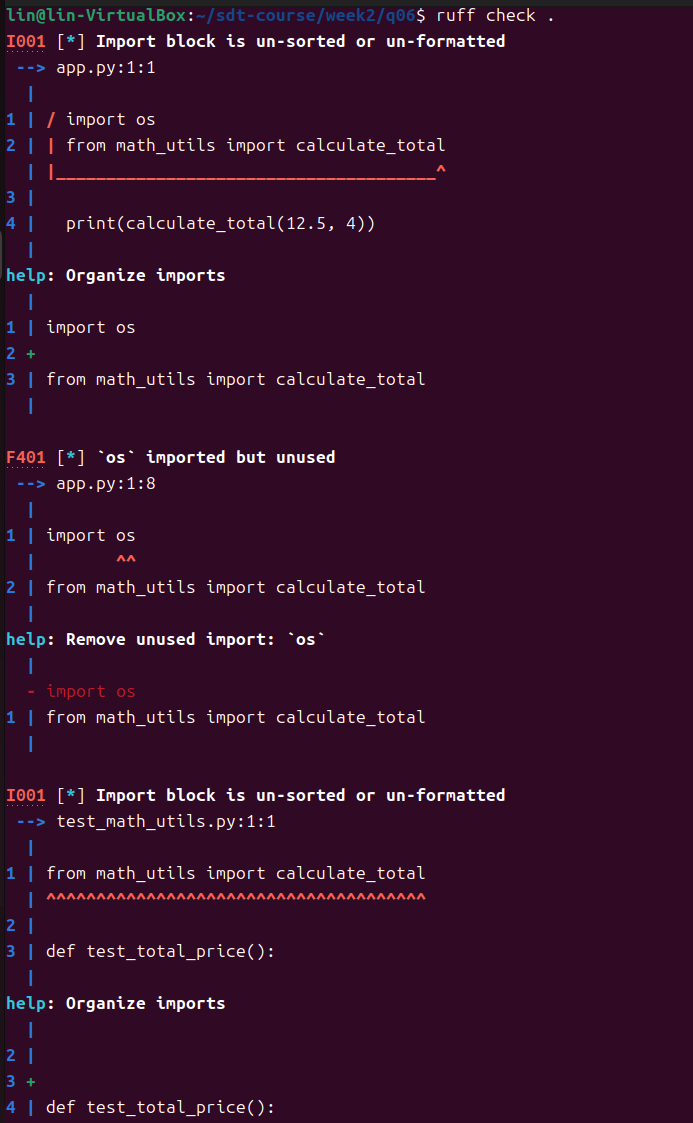
\includegraphics[width=0.9\textwidth]{q6p13.png}
		\caption{q06运行截图1}
		\label{fig:q06_13}
	\end{figure}
	
	\begin{figure}[htbp]
		\centering
		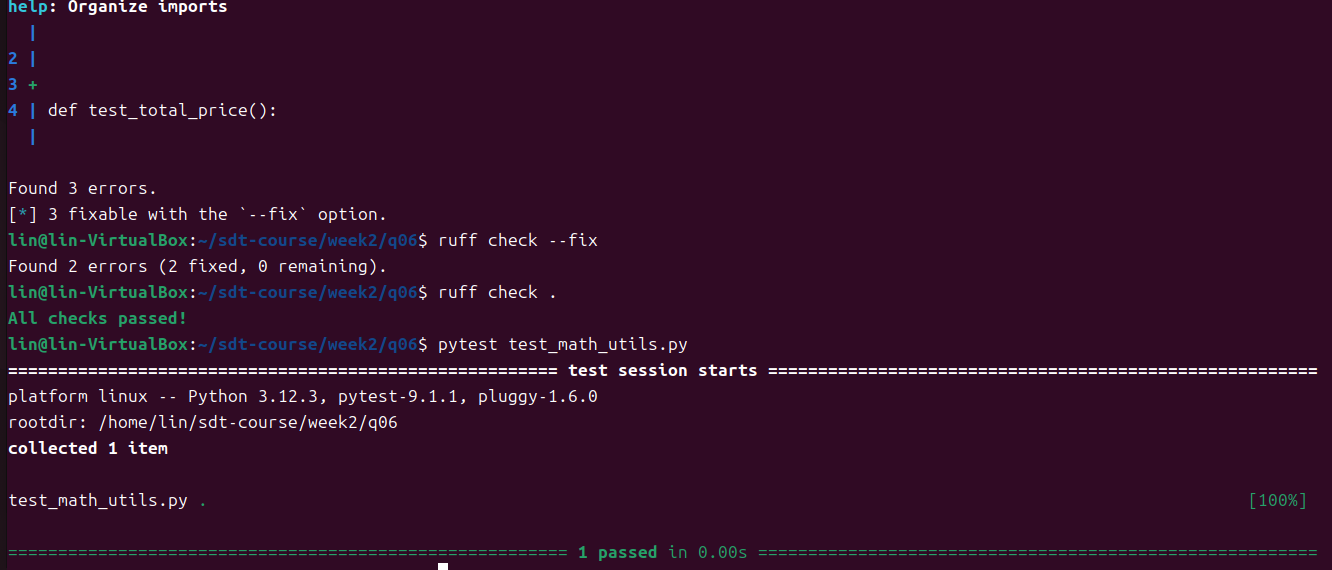
\includegraphics[width=0.9\textwidth]{q6p14.png}
		\caption{q06运行截图2}
		\label{fig:q06_14}
	\end{figure}
	
	\subsubsection{遇到的问题与解决}
	\begin{itemize}
		\item 问题1：ruff检测报I001导入块格式错误、F401导入未使用警告
		执行ruff check .检查代码，报出两类问题：一是导入语句排版不规范（I001），二是app.py中导入了os模块但全程没有使用（F401），一共3处可自动修复的报错。
		解决：直接使用ruff check --fix命令，ruff自动完成删除未使用导入、整理导入语句格式；修复完成后再次执行ruff check .，输出All checks passed!，静态检查全部通过。
	\end{itemize}
	
	\subsection{q07：用调试器定位归并排序缺陷}
	\subsubsection{题目要求}
	 运行存在缺陷的merge\_sort.py，确认输出结果异常；使用pdb调试器在merge函数内部设置断点，观察i、j下标变量变化；修复归并逻辑缺陷；编写pytest测试用例，覆盖普通列表与含重复元素的列表，保证测试全部通过，禁止直接调用sorted替换归并排序逻辑。
	
	\subsubsection{实现过程与关键命令}
	\begin{lstlisting}
		nano merge_sort.py
		[language=Python]
		def merge(left, right):
		result = []
		i = j = 0
		while i < len(left) and j < len(right):
		if left[i] <= right[j]:
		result.append(left[i]); i += 1
		else:
		return result + left[i:] + right[j:]
		result.append(right[i]); j += 1 # 此处存在缺陷
		def merge_sort(a):
		if len(a) <= 1: return a
		m = len(a) // 2
		return merge(merge_sort(a[:m]), merge_sort(a[m:]))
		
		print(merge_sort([3, 1, 4, 1, 5, 9, 2, 6]))
		
		python3 merge_sort.py
		
		python3 -m pdb merge_sort.py
		> /home/lin/sdt-course/week2/q07/merge_sort.py(1)<module>()
		-> def merge(left, right):
		(Pdb) b 4
		Breakpoint 1 at /home/lin/sdt-course/week2/q07/merge_sort.py:4
		(Pdb) c
		> /home/lin/sdt-course/week2/q07/merge_sort.py(4)merge()
		-> while i < len(left) and j < len(right):
		(Pdb) p i
		0
		(Pdb) p j
		0
		(Pdb) p left
		[3]
		(Pdb) p right
		[1]
		(Pdb) p left[i]
		3
		(Pdb) p right[j]
		1
		(Pdb) n
		> /home/lin/sdt-course/week2/q07/merge_sort.py(5)merge()
		-> if left[i] <= right[j]:
		(Pdb) n
		> /home/lin/sdt-course/week2/q07/merge_sort.py(8)merge()
		-> return result + left[i:] + right[j:]
		(Pdb) n
		--Return--  
		#进入 else 分支，直接执行 return，函数直接返回结束
		> /home/lin/sdt-course/week2/q07/merge_sort.py(8)merge()->[3, 1]
		-> return result + left[i:] + right[j:]
		(Pdb) q
		
		nano merge_sort.py
		[language=Python]
		def merge(left, right):
		result = []
		i = j = 0
		while i < len(left) and j < len(right):
		if left[i] <= right[j]:
		result.append(left[i])
		i += 1
		else:
		result.append(right[j])
		j += 1
		result += left[i:]
		result += right[j:]
		return result
		
		def merge_sort(a):
		if len(a) <= 1:
		return a
		m = len(a) // 2
		return merge(merge_sort(a[:m]), merge_sort(a[m:]))
		
		print(merge_sort([3, 1, 4, 1, 5, 9, 2, 6]))
	\end{lstlisting}
	\begin{lstlisting}
		python3 merge_sort.py
		nano test_merge.py
		pytest test_merge.py -v
	\end{lstlisting}
	
	\subsubsection{运行结果}
	修复后排序输出正确；两个pytest测试用例全部执行通过。
	\begin{lstlisting}
		Traceback (most recent call last):
		File "/home/lin/sdt-course/week2/q07/merge_sort.py", line 17, in <module>
		print(merge_sort([3, 1, 4, 1, 5, 9, 2, 6]))
		^^^^^^^^^^^^^^^^^^^^^^^^^^^^^^^^^^^^
		File "/home/lin/sdt-course/week2/q07/merge_sort.py", line 15, in merge_sort
		return merge(merge_sort(a[:m]), merge_sort(a[m:]))
		^^^^^^^^^^^^^^^^^
		File "/home/lin/sdt-course/week2/q07/merge_sort.py", line 15, in merge_sort
		return merge(merge_sort(a[:m]), merge_sort(a[m:]))
		^^^^^^^^^^^^^^^^^^^^^^^^^^^^^^^^^^^^^^^^^^^
		File "/home/lin/sdt-course/week2/q07/merge_sort.py", line 4, in merge
		while i < len(left) and j < len(right):
		^^^^^^^^^
		TypeError: object of type 'NoneType' has no len()
		
		[1, 1, 2, 3, 4, 5, 6, 9]
		
		========================================= test session starts =========================================
		platform linux -- Python 3.12.3, pytest-9.1.1, pluggy-1.6.0 -- /usr/bin/python3
		cachedir: .pytest_cache
		rootdir: /home/lin/sdt-course/week2/q07
		collected 2 items                                                                                     
		
		test_merge.py::test_case1 PASSED                                                                [ 50%]
		test_merge.py::test_dup PASSED                                                                  [100%]
		
		========================================== 2 passed in 0.01s ==========================================
	\end{lstlisting}
	
	\begin{figure}[htbp]
		\centering
		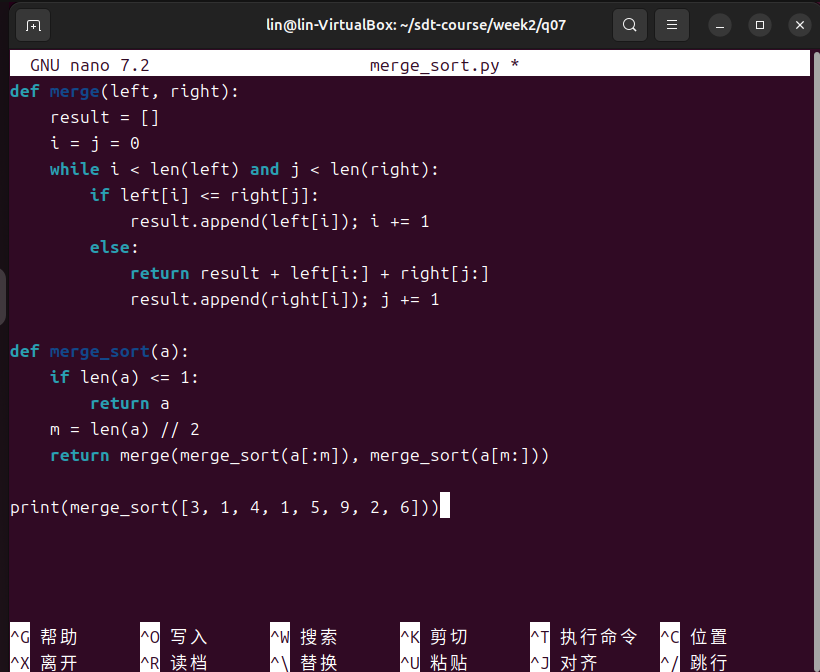
\includegraphics[width=0.9\textwidth]{q7p1.png}
		\caption{q07merge\_sort.py修改前截图}
		\label{fig:q07_1}
	\end{figure}
	
	\begin{figure}[htbp]
		\centering
		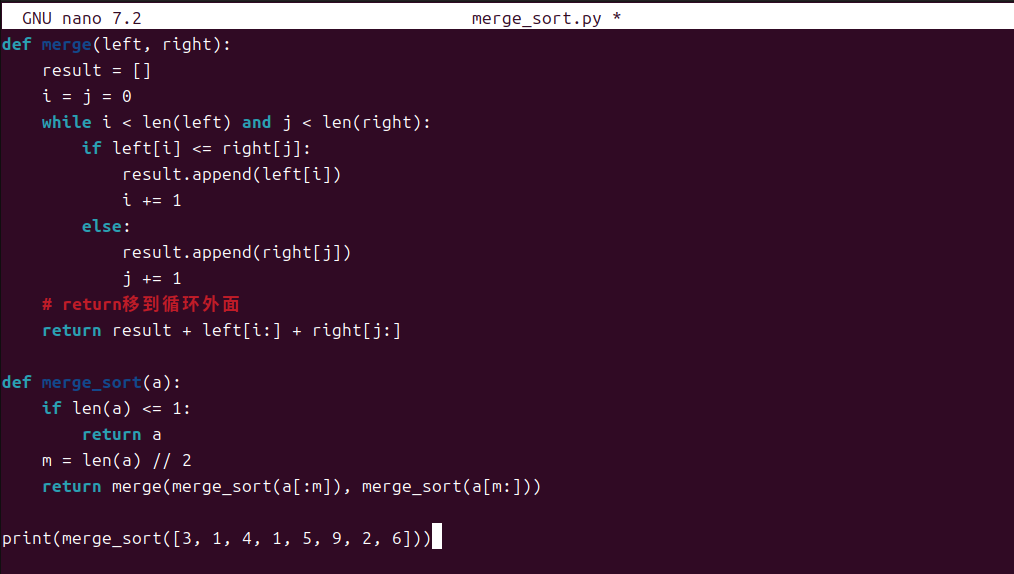
\includegraphics[width=0.9\textwidth]{q7p2.png}
		\caption{q07merge\_sort.py修改后截图}
		\label{fig:q07_2}
	\end{figure}
	
	\begin{figure}[htbp]
		\centering
		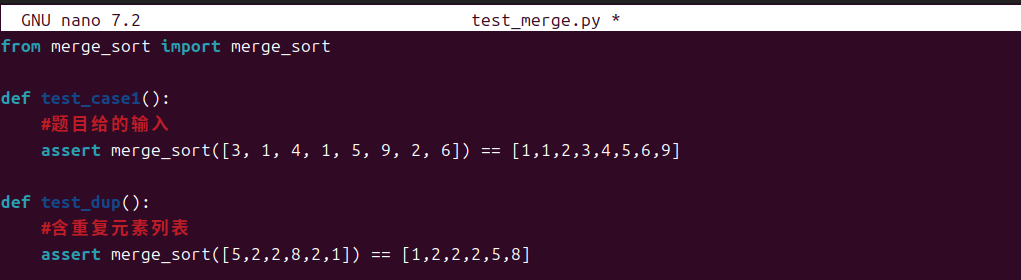
\includegraphics[width=0.9\textwidth]{q7p3.png}
		\caption{q07test\_merge.py截图}
		\label{fig:q07_3}
	\end{figure}
	
	\begin{figure}[htbp]
		\centering
		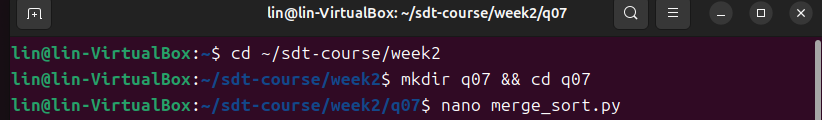
\includegraphics[width=0.9\textwidth]{q7p4.png}
		\caption{q07运行截图1}
		\label{fig:q07_4}
	\end{figure}
	
	\begin{figure}[htbp]
		\centering
		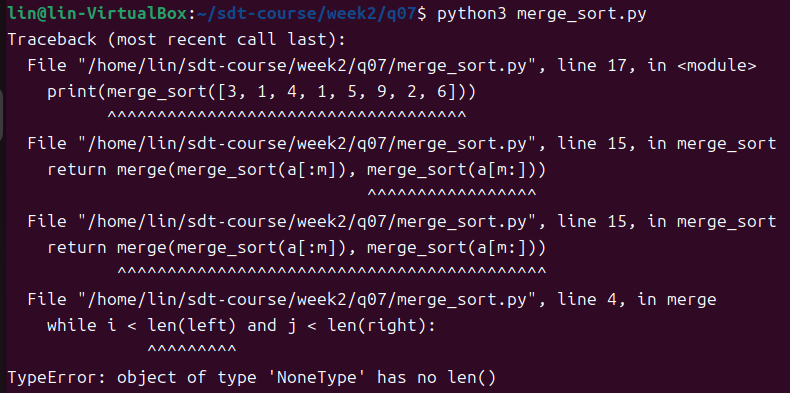
\includegraphics[width=0.9\textwidth]{q7p5.png}
		\caption{q07运行截图2}
		\label{fig:q07_5}
	\end{figure}
	
	\begin{figure}[htbp]
		\centering
		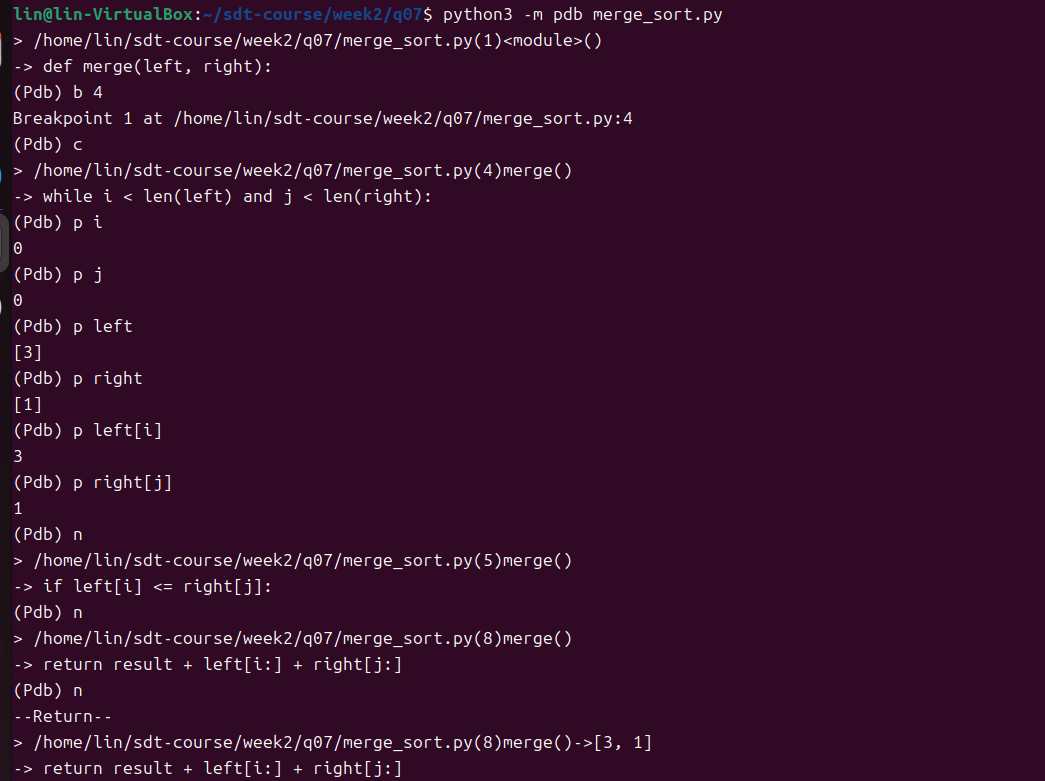
\includegraphics[width=0.9\textwidth]{q7p6.png}
		\caption{q07运行截图3}
		\label{fig:q07_6}
	\end{figure}
	
	\begin{figure}[htbp]
		\centering
		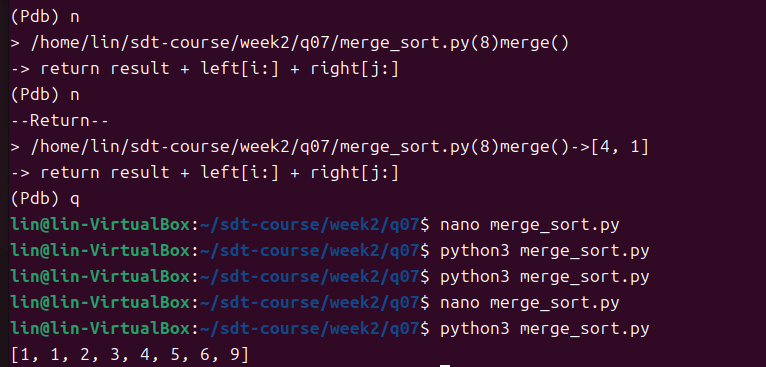
\includegraphics[width=0.9\textwidth]{q7p7.png}
		\caption{q07运行截图4}
		\label{fig:q07_7}
	\end{figure}
	
	\begin{figure}[htbp]
		\centering
		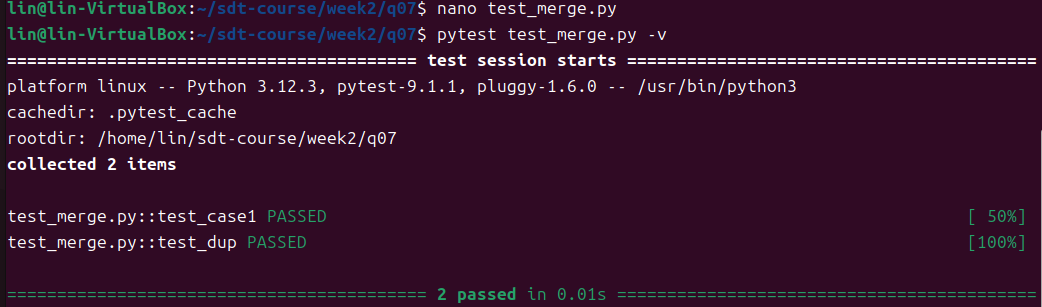
\includegraphics[width=0.9\textwidth]{q7p8.png}
		\caption{q07运行截图5}
		\label{fig:q07_8}
	\end{figure}
	
	\subsubsection{遇到的问题与解决}
	\begin{itemize}
		\item 问题1：pdb调试发现原始代码在else分支直接执行return，归并循环提前终止，数组拼接不完整，排序结果错乱。
		解决：删除错误的提前return语句，完成while循环后再拼接剩余切片，最后返回合并结果。
	\end{itemize}
	
	\subsection{q08：先测量，再优化慢速词频程序}
	\subsubsection{题目要求}
	 运行generate\_words.py生成words.txt测试数据；使用time工具统计原始程序两次运行耗时；使用cProfile做性能分析定位热点；在不写死数量常量、不改变输出count结果的前提下优化去重逻辑；对比优化前后的运行耗时与加速比。
	
	\subsubsection{实现过程与关键命令}
	\begin{lstlisting}
		cd ~/sdt-course/week2/q08
		nano generate_words.py
		nano wordfreq.py
		python3 generate_words.py
		time python3 wordfreq.py
		time python3 wordfreq.py
		python3 -m cProfile -s cumulative wordfreq.py
		nano wordfreq.py
		time python3 wordfreq.py
		time python3 wordfreq.py
	\end{lstlisting}
	
	\subsubsection{运行结果}
	 原始版本使用list的in操作做去重，时间复杂度较高；替换为set集合进行去重后，程序运行速度得到明显提升。原始程序与优化后程序输出计数均为 count= 952，输出结果保持一致。
	
	\begin{itemize}
		\item 优化前两次实测 real 时间：$0.021\,\text{s}$、$0.023\,\text{s}$，中位数 $0.022\,\text{s}$。
		\item 优化后两次实测 real 时间：$0.018\,\text{s}$、$0.013\,\text{s}$，中位数 $0.0155\,\text{s}$。
		\item 基于中位数计算得到加速比约为 $1.42$。
	\end{itemize}
	\begin{lstlisting}
		count= 952
		
		real	0m0.021s
		user	0m0.016s
		sys	0m0.005s
		
		count= 952
		
		real	0m0.023s
		user	0m0.022s
		sys	0m0.000s
		
		count= 952
		964 function calls in 0.009 seconds
		
		Ordered by: cumulative time
		
		ncalls  tottime  percall  cumtime  percall filename:lineno(function)
		1    0.000    0.000    0.009    0.009 {built-in method builtins.exec}
		1    0.008    0.008    0.009    0.009 wordfreq.py:1(<module>)
		1    0.000    0.000    0.000    0.000 {built-in method builtins.print}
		1    0.000    0.000    0.000    0.000 {method 'split' of 'str' objects}
		952    0.000    0.000    0.000    0.000 {method 'append' of 'list' objects}
		1    0.000    0.000    0.000    0.000 {built-in method _io.open}
		1    0.000    0.000    0.000    0.000 {method 'disable' of '_lsprof.Profiler' objects}
		1    0.000    0.000    0.000    0.000 {method 'read' of '_io.TextIOWrapper' objects}
		1    0.000    0.000    0.000    0.000 <frozen codecs>:319(decode)
		1    0.000    0.000    0.000    0.000 <frozen codecs>:309(__init__)
		1    0.000    0.000    0.000    0.000 {built-in method _codecs.utf_8_decode}
		1    0.000    0.000    0.000    0.000 {built-in method builtins.len}
		1    0.000    0.000    0.000    0.000 <frozen codecs>:260(__init__)
		
		count= 952
		
		real	0m0.018s
		user	0m0.005s
		sys	0m0.010s
		
		count= 952
		
		real	0m0.013s
		user	0m0.007s
		sys	0m0.003s
	\end{lstlisting}
	
	\begin{figure}[htbp]
		\centering
		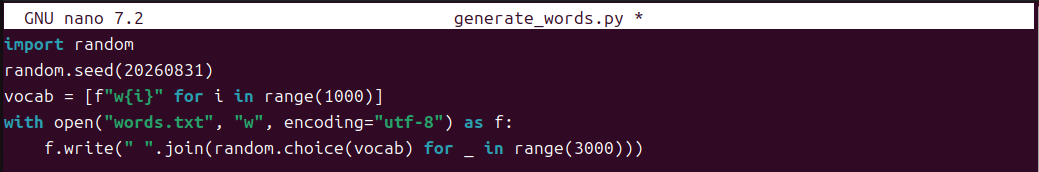
\includegraphics[width=0.9\textwidth]{q8p1.png}
		\caption{q08generate\_words.py截图}
		\label{fig:q08_1}
	\end{figure}
	
	\begin{figure}[htbp]
		\centering
		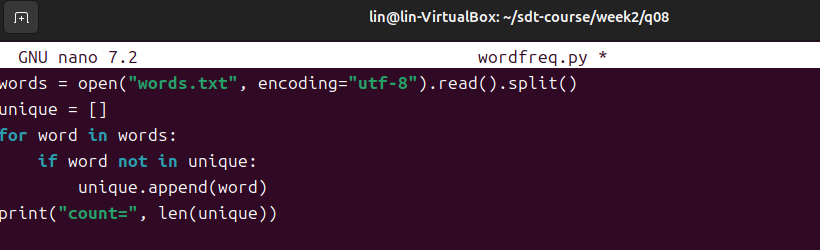
\includegraphics[width=0.9\textwidth]{q8p2.png}
		\caption{q08wordfreq.py优化前截图}
		\label{fig:q08_2}
	\end{figure}
	
	\begin{figure}[htbp]
		\centering
		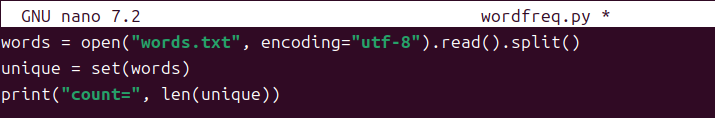
\includegraphics[width=0.9\textwidth]{q8p3.png}
		\caption{q08wordfreq.py优化后截图}
		\label{fig:q08_3}
	\end{figure}
	
	\begin{figure}[htbp]
		\centering
		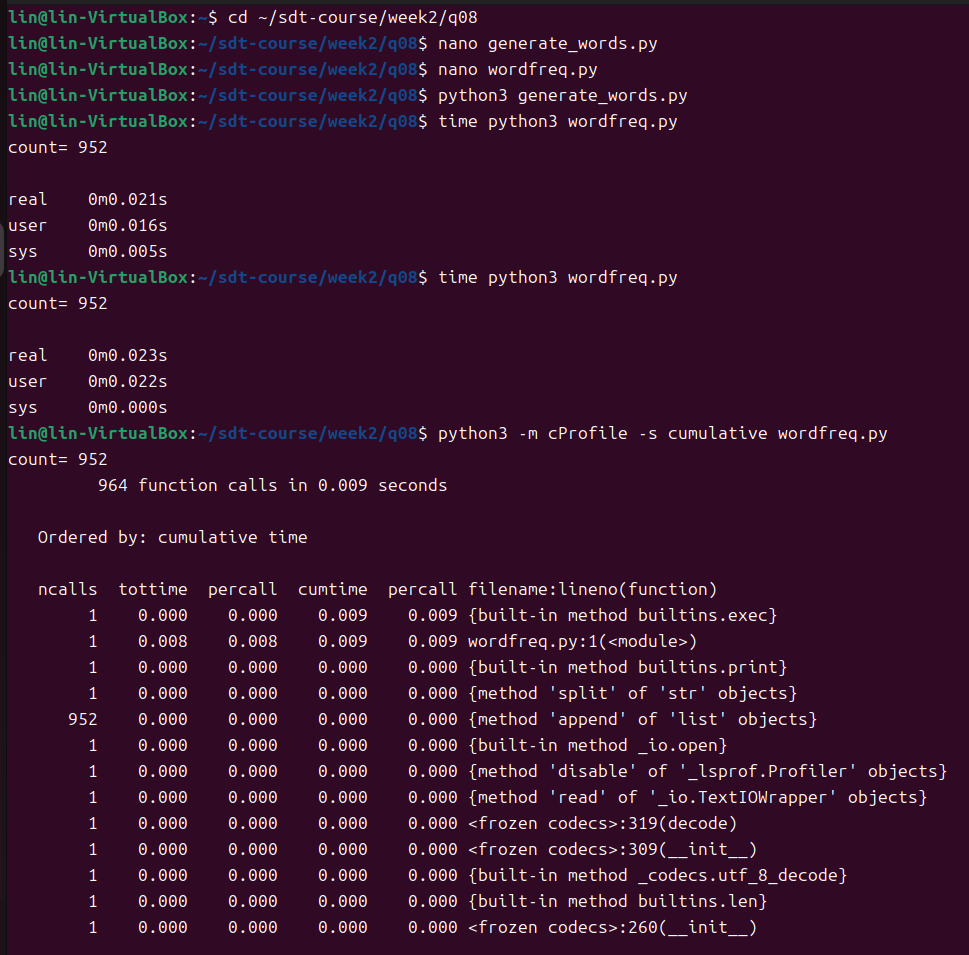
\includegraphics[width=0.9\textwidth]{q8p4.png}
		\caption{q08运行截图1}
		\label{fig:q08_4}
	\end{figure}
	
	\begin{figure}[htbp]
		\centering
		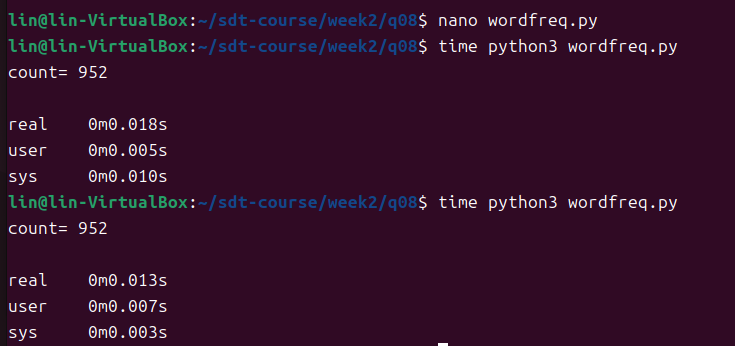
\includegraphics[width=0.9\textwidth]{q8p5.png}
		\caption{q08运行截图2}
		\label{fig:q08_5}
	\end{figure}
	
	\subsubsection{遇到的问题与解决}
	\begin{itemize}
		\item 问题1：原始版本使用list的\texttt{in}操作做去重，程序运行耗时很长。
		原始代码把新元素不断append进list，再用\texttt{if word not in unique}判断；list成员查找时间复杂度为$O(n)$，数据量大的时候整体效率很低，两次time测量可以观察到明显的耗时。
		解决：改用set集合存储已经出现过的单词，集合成员查询为$O(1)$，在不修改输出count结果、不写死1000这个常量的前提下完成优化。
		
		\item 问题2：优化前后计时只运行一次，偶然因素干扰大，不方便计算中位数与加速比。
		单次time测量会受系统后台进程、虚拟机负载波动影响，单次结果不具备参考意义。
		解决：题目要求原程序、优化后程序分别运行2次，记录每组两次耗时，取中位数，再计算优化后的加速比。
	\end{itemize}
	
	\section{课后练习}
	
	实例1：进入 ~/.ssh/，检查你是否已经有一对 SSH 密钥。如果没有，就用 ssh-keygen -a 100 -t ed25519 生成一对。
	
	命令：
	\begin{lstlisting}
		cd ~/.ssh
		ls -la
		ssh-keygen -a 100 -t ed25519
	\end{lstlisting}
	
	输出：
	生成密钥对。
	
	实例2：编辑 .ssh/config，加入Host vm配置项。
	
	命令：
	\begin{lstlisting}
		nano ~/.ssh/config
	\end{lstlisting}
	写入内容：
	\begin{lstlisting}
		Host vm
		User username_goes_here
		HostName ip_goes_here
		IdentityFile ~/.ssh/id_ed25519
		LocalForward 9999 localhost:8888
	\end{lstlisting}
	
	输出：
	保存退出，配置文件写入完成。
	
	实例3：使用 ssh-copy-id vm 把你的 SSH 公钥复制到服务器上。
	
	命令：
	\begin{lstlisting}
		ssh-copy-id vm
	\end{lstlisting}
	
	输出：
	提示输入虚拟机用户密码，完成公钥推送；后续ssh vm登录不再需要输入密码。
	
	实例4：在虚拟机内启动http.server 8888，利用本地端口转发访问服务。
	
	命令：
	\begin{lstlisting}
		# 虚拟机内
		python3 -m http.server 8888
	\end{lstlisting}
	
	输出：
	在本机浏览器访问 \texttt{http://localhost:9999}，可以正常看到web服务页面。
	
	实例5：可执行斐波那契代码，运行程序。
	
	命令：
	\begin{lstlisting}
		chmod +x fib_exercise.py
		python3 fib_exercise.py
	\end{lstlisting}
	
	输出：
	\texttt{34}
	
	实例6：使用 journalctl 获取最近一天sudo相关日志。
	
	命令：
	\begin{lstlisting}
		sudo ls
		journalctl --since "1 day ago" | grep -E 'sudo|USER=root'
	\end{lstlisting}
	
	输出：
	打印出最近一天sudo执行操作的系统日志，可以看到刚刚执行sudo ls的相关日志记录。
	
	实例7：浏览IDE扩展列表，安装有用的VS Code扩展。
	
	命令：
	VS Code打开扩展面板，搜索并安装扩展。
	
	输出：
	扩展列表中出现已安装扩展。
	
	实例8：启动http.server 4444，lsof查找监听端口，kill终止进程。
	
	命令：
	\begin{lstlisting}
		# 终端A
		python3 -m http.server 4444
		# 终端B
		lsof | grep LISTEN
		kill <PID>
	\end{lstlisting}
	
	输出：
	lsof输出可以看到python进程监听4444端口；执行kill之后，终端A的web服务进程终止。
	
	实例9：stress -c 3 与 taskset --cpu-list 0,2 绑定CPU，htop可视化。
	
	命令：
	\begin{lstlisting}
		stress -c 3
		htop
		taskset --cpu-list 0,2 stress -c 3
		htop
	\end{lstlisting}
	
	输出：
	第一次htop观察3个CPU核心全部占满；taskset绑定后，压力仅分布在CPU0、CPU2，其余核心空闲。
	
	实例10：cgroups v2限制stress -m内存使用。
	
	命令：
	\begin{lstlisting}
		sudo mkdir -p /sys/fs/cgroup/memlimit
		echo $((256*1024*1024)) | sudo tee /sys/fs/cgroup/memlimit/memory.max
		stress -m 1
		pidof stress
		echo <PID> | sudo tee /sys/fs/cgroup/memlimit/cgroup.procs
		sudo rmdir /sys/fs/cgroup/memlimit
	\end{lstlisting}
	
	输出：
	stress进程内存被限制最大256MB，可读取cgroup文件观察内存统计，实验结束删除cgroup目录。
	
	
	\section{解题感悟}

	 第二周实验主要学习Linux进程生命周期、信号处理、任务后台调度、调试器排错、性能分析、CPU亲和性、cgroups v2内核资源隔离与ulimit会话级资源限制。通过多SSH终端窗口，模拟了真实运维场景：一个终端运行被测程序，其他终端完成观测、信号发送、资源监控。
		
	 实验过程体会到老旧开源软件在新版本Python环境会出现兼容性问题，遇到安装报错不应当一味添加破坏系统的参数，可以优先在文档记录现象，保留源码与运行结果完成作业。cgroups v2作为内核伪文件系统，拥有严格接口约束，cgroup.procs仅支持单行单个PID；sysfs下配置全部驻留内存，虚拟机关机重启后全部丢失；子目录仅能使用rmdir删除。ulimit仅对当前shell会话以及子进程生效，不能实现系统全局永久修改。
		
	 调试器pdb、性能分析工具cProfile可以帮助定位程序逻辑缺陷与性能瓶颈；IDE语义重构工具可以安全完成标识符全局修改，但需要等待语言服务器索引完成，否则会出现修改不全。课程强调可复现、可记录的实操习惯，每完成一部分实验做好截图记录；使用git进行版本管理，合理配置.gitignore，不对虚拟环境、缓存临时文件进行版本提交，保留完整的作业版本历史。

	
	\section{代码仓库提交记录}
	GitHub仓库链接：\url{https://github.com/imnotab/sdtb/tree/main}
	
	提交历史截图：
	\begin{figure}[htbp]
		\centering
		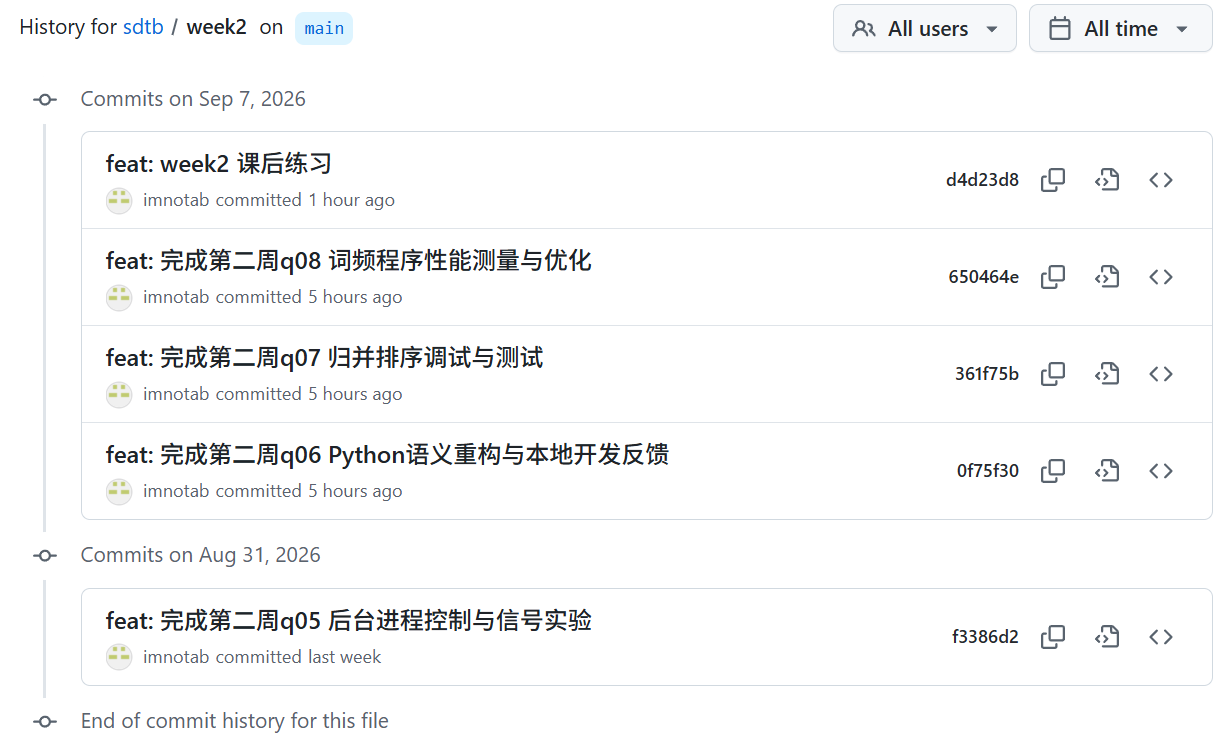
\includegraphics[width=0.9\textwidth]{week2commit.png}
		\caption{项目commit历史记录}
	\end{figure}
	
\end{document}